\documentclass[12pt]{article}

\usepackage{lmodern}
\usepackage[T1]{fontenc}
\usepackage[spanish,activeacute]{babel}
\usepackage{mathtools}
\usepackage[utf8]{inputenc}

\title{
	ESTEGANOGRAFIA POR TRANSORMADA RÁPIDA DE FOURIER PARA RECONOCER LA AUTENTICIDAD DE UNA IMAGEN PRODUCIDA POR UN DISPOSITIVO CON UN SISTEMA OPERATIVO ANDROID
}

\author{Oscar Flores Bobadilla}

\begin{document}
% cuerpo del documento

%*****************creación de la carátula*******************
\begin{center}

\includegraphics[width = 2cm]{itt.png}
\begin{Huge}
\textbf{\large INSTITUTO TECNOLÓGICO DE TOLUCA} \ \\ \ \\  %
\end{Huge}
\end{center}

\begin{center}
\begin{Huge}
\textbf{\large ESTEGANOGRAFIA CON FFT PARA RECONOCER LA AUTENTICIDAD DE UNA IMAGEN} \ \\ \ \\  %
\end{Huge}
\end{center}

\begin{center}
\begin{Huge}
\textsc{\Large Taller de Investigación II} \ \\ \ \\ \ \\ %
\end{Huge}
\end{center}

\begin{center}
\begin{Huge}
\textsc{\Large Carrera:}
\end{Huge}
\end{center}

\begin{center}
\begin{Huge}
\textsc{\Large Ingeniería en Sistemas Computacionales} \ \\ \ \\  %
\end{Huge}
\end{center}

\begin{center}
\begin{Huge}
\textsc{\Large Asesor:} 
\end{Huge}
\end{center}

\begin{center}
\begin{Huge}
\textsc{\Large Dra. Eréndira Rendón Lara} \ \\ \ \\  %
\end{Huge}
\end{center}

\begin{center}
\begin{Huge}
\textsc{\Large Presenta:}
\end{Huge}
\end{center}

\begin{center}
\begin{Huge}
\textsc{\Large Oscar Flores Bobadilla}
\end{Huge}
\end{center}
%fin caratula

\maketitle
\newpage

\tableofcontents
\newpage
\listoffigures
\newpage
\section{Capitulo I: Introducion}
\subsection{Antecedentes.}
La esteganografía ha despertado mucho interés en los últimos años debido a que ha sido utilizada por organizaciones criminales y terroristas  ya  que trata el estudio y aplicación de técnicas que permiten ocultar mensajes u objetos, dentro de otros, llamados portadores, de modo que no se perciba su existencia, pero para nuestros fines no se realizara ningún acto perjudicial. No obstante, no se trata de ningún nuevo ingenio, se lleva empleando desde la más remota antigüedad. Cabe resaltar que la esteganografía ha estado presente en nuestra civilización desde tiempos inmemoriales y ha sido tradicionalmente empleada por las agencias militares.

Ahora bien, mientras la estenografía clásica se basaba únicamente en el desconocimiento del canal de información encubierto, en la era moderna se emplean canales digitales (imagen, video, audio, etc.) para alcanzar el objetivo. En muchos casos el objeto contenedor es conocido como en nuestro caso, pero lo que se ignora es el “algoritmo de inserción” de la información en dicho objeto. Como ejemplo se puede citar algoritmo de la marca de agua inteligente aplicado al dinero Electrónico para proteger los derechos del autor publicado en el 5º Congreso Ibero-Americano sobre Información de Seguridad por Jaimes, Patricia (2009).\cite{Jaimes}

Hay varias formas de saber sí una fotografía es auténtica o falsa desde metidos rudimentarios como percibir anomalías con el ojo humano o hacer comparaciones de muchas imágenes por medio de servidores como TINEYE, hasta usar a los metadatos de una Foto digital para saber si esta ha sido editado por algún software, pero estos metadatos son fácilmente editables por programas como EXIF por mencionar alguno.

Para olvidarnos del riesgo de que alguna imagen sea manipulada para mostrar cosas que no sucedieron o para no mostrar las que sí ocurrieron, se impone el esquema de selección por umbral de entropía (ET) donde Carlos L. Velasco Bautista y colaboradores (2007) nos dicen que se usa la energía de una imagen para determinar si se inserta el mensaje secreto o no. Solo bloques con mayor energía que el valor de umbral determinado anteriormente son usados para ocultar el mensaje secreto. Pero esta técnica no es muy usada puesto que solo se puede usar en imágenes de escala de grises.\cite{Velasco}

A su vez Yusuke Lim, y colaboradores (2001) propusieron un autenticador de imágenes basado en web, usando marcas de aguas invisibles, conocidas como frágiles. Cualquier usuario autorizado podía generar una imagen con una marca de agua, también podía verificar la autenticidad de la imagen. Intentaron usar “secure socket layer (SSL)” para asegurar acceso al servidor, pero fue dejado como trabajo futuro. \cite{Yusuk}

Para cualquier formato convencional de imagen se puede usar una herramienta para el procesamiento de imágenes digitales conocida  como Transformada Discreta de Fourier porque es posible implementarse en diversos entornos de desarrollo. Así lo menciona Ramos B. (2004) en su artículo titulado “Encriptamiento de imágenes digitales a color mediante Transformada de Fourier”. \cite{Ramos}

\subsection{Definición del Problema.}
El demostrar que la autenticidad de una imagen digital sea verdadera no es una tarea fácil y menos si ésta esta fue producida a base de un dispositivo móvil. Actualmente existen muchas herramientas computacionales que permiten falsificar Imagines. El objetivo de la investigación consiste en desarrollar un mecanismo esteganográfico que permita codificar un mensaje de autenticidad directamente en la imagen y, así mismo, decodificarlo para identificar la autenticidad de la imagen. Con lo cual se podrá conocer la autenticidad de dicha imagen.

\subsection{Objetivos.}
\subsubsection{Objetivo General.}
Desarrollar un sistema esteganográfico de inserción de mensaje oculto basado en la trasformada rápida de Fourier. El mensaje oculto será insertado en una imagen inmediatamente que ha sido producida por la cámara de un dispositivo móvil.

\subsubsection{Objetivos Específicos.}
\begin{itemize}
\item Comprender el algoritmo de inserción basado en la Transformada Rápida de Fourier. Ya que este se puede implementar en imágenes de gran tamaño con variedades de colores.
\item Implementar el algoritmo para insertar en una imagen un mensaje de Autenticidad.
\item Implementar un algoritmo que será usado para reconocer el mensaje de Autenticidad en un momento dado.
\item Implementar los algoritmos para desarrollar un sistema para dispositivos  móviles con sistema operativo Android.
\end{itemize}

\subsection{Justificación.}
El sistema que se va a desarrollar tiene el propósito de brindar a  la gente la confianza de estar seguro de lo que ve a través del popular medio de comunicación llamado Internet, puesto que cada día miles de nuevas fotografías circulan las redes sociales. Un porcentaje de ellas son montajes completamente falsos y cuando se trata de una persona degradan su integridad como ser humano. Y los argumentos que ahí se expresan no son nada útiles para minimizar la vergüenza que esta pueda generar al individuo involucrado.

Además muchas veces son Intereses políticos o económicos son los que incitan a modificar la verdad por medio de una imagen. Otra causa puede ser el afán de engañar a los medios de comunicación o una simple broma de mal gusto.

\subsection{Hipótesis.}
Cuando se ha insertado un mensaje oculto a una Imagen de gran tamaño con variedades de colores y si se utiliza un método de inserción basado En la Transformada Rápida de Fourier, entonces se logrará ocultar el mensaje. Posteriormente si esta se edita aunque sea un pixel, entonces el mensaje oculto se destruirá. El mensaje de destruye porque la imagen necesita hacer sumatorias con cada unos de sus pixeles: cada letra del texto a esconder se asemeja la composición RGB de un pixel, es por eso que al editar un pixel de la imagen, este se combinara con el texto oculto al realizar La trasformada Rápida de Fourier Inversa y el texto oculto no podrá asimilarse en la posición que le corresponde. Por ende la perdida de datos de la imagen dependerá del número de bits insertados: por ejemplo, si tuviéramos una imagen de 8*8 pixeles (64 bits) y se insertara 1 bit, entonces la perdida sería de 0.64 \%.

\subsection{Organización de Actividades.}
En el próximo capítulo se detallarán los conceptos básicos necesarios para comprender  el presente trabajo, es decir se describirá el Marco Teórico. De la misma manera, se podrán descubrir los trabajos posteriores  de la estenografía en el “Estado del Arte”. Posteriormente, en el capítulo 3 se explicará la metodología en profundidad, para dar solución al problema planteado. Y para finalizar se expresaran las conclusiones y experimentos realizados en la investigación.

\newpage
\section{Capitullo II: Marco Teórico.}

\subsection{Esteganografía:}
La palabra esteganografía proviene del griego y cuyo significado es: “escrito protegido” se utiliza para denominar a la ciencia que estudia la ocultación de información en otra información. La esteganografía actual trata de esconder datos de bits que suponen un archivo. Los bits que componen el mensaje a ocultar se introducen (ya sea añadiéndolos, o realizando operaciones aritméticas con los datos originales) en el archivo ya existente, procurando que el archivo resultante después de realizar los cambios tenga un alto parecido con el original. La esteganografía utiliza un medio digital como archivos de texto, audio, imagen y video que son utilizados como un archivo de transporte, para ocultar la información. A este medio se le conoce como contenedor o cubierta y tiene la característica de que ser un contenedor aparentemente inocente que no despierte ninguna sospecha. \cite{Chavez}
\newline
\begin{figure}[hbtp]
\centering
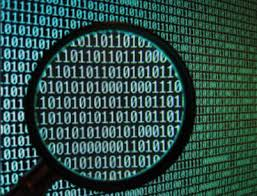
\includegraphics[width = 5cm]{esteganografia.jpeg}
\caption{Información oculta}
\end{figure}

\subsection{Transformada Rápida de Fourier (DFT)}
Uno de los algoritmos más ampliamente utilizados es la transformada rápida de Fourier, un medio eficaz de ejecutar un cálculo matemático básico y de frecuente empleo. La transformada de Fourier es de es de importancia fundamental para el análisis matemático y ha sido objeto de numerosos estudios. La aparición de un algoritmo eficaz para esta operación fue una piedra angular para la historia de la informática.

Las siguientes ecuaciones proporcionan las definiciones matemáticas de las DFT y IDFT (Transformada de Fourier Discreta Inversa) para vectores de números lineales, así, la transformada X está dada por:
\newline
\textbf {
	$X_k = \sum_{n=0}^{N-1}x_ne^{\frac{2{\pi}i}{N}kn}, k = 0,..., N - 1$
}
\newline
y su transformada  inversa x:
\newline
\textbf {
	$x_n = \frac{1}{N}\sum_{k=0}^{N-1}X_ke^{\frac{2{\pi}i}{N}kn}, n = 0,..., N - 1$
}
\newline
\cite{Sedgewic}

\subsection{Transformada discreta del coseno (DCT)}
La transformada DCT es una transformada semejante a la transformada rápida de Fourier, ésta toma un conjunto de puntos de un dominio espacial y los transforma en una representación equivalente en el dominio de frecuencias. La DCT está bastante relacionada con la DFT, con la diferencia de que es una transformada real, debido a que los vectores base se componen exclusivamente de funciones coseno muestreadas. La transformada discreta de coseno es la más ampliamente utilizada en compresión de imágenes y videos. Esta transformada cuenta con una buena propiedad de compactación de energía, que produce coeficientes incorrelados, es decir que no implica dependencia, donde los vectores base de la DCT dependen sólo del orden seleccionado de la transformada y no de las propiedades estadísticas de los datos de entrada.

Las siguientes ecuaciones proporcionan las definiciones matemáticas de las DCT y IDCT (Transformada Discreta Inversa del Coseno) de un bloque de 8x8 de una imagen f, así, la transformada F está dada por:
\newline
\textbf {
	$F(u, v) = \frac{1}{4}C(u)C(v)[\sum_{x=0}^{7}\sum_{y=0}^{7}f(x, y)cos \frac{(2x + 1)u\pi}{16}cos \frac{(2y + 1)v\pi}{16}]$
}
\newline
y su transformada  inversa f:
\newline
\textbf {
	$f(u, v) = \frac{1}{4}[\sum_{x=0}^{7}\sum_{y=0}^{7}C(u)C(v)F(x, y)cos \frac{(2x + 1)u\pi}{16}cos \frac{(2y + 1)v\pi}{16}]$
}
\newline
\cite{Esqueda}
\newpage


\subsection{Algoritmo de inserción.}

\begin{enumerate}
\item La imagen se divide en bloques de 8x8 píxeles.
\item Se aplica la FFT (Transformada Rápida de Fourier) a todos los bloques de la imagen.
\item Los coeficientes de FFT de cada bloque es dividido por la matriz de cuantificación [Mfc].
\item Se hace un escaneo en zigzag a cada bloque seleccionado, obteniendo un vector de longitud 64.
\item Se considera la banda de baja frecuencia para la inserción del mensaje secreto (i.e., 1 < k < n). Aquí n<64.
\item El valor absoluto de cada coeficiente cij es redondeado,
\item rk = |round (cij)|, 1 < k < n
\item Si rk > t, entonces al bit menos significativo del coeficiente ck se le inserta un bit del mensaje secreto.
\item Se reordena el vector a una matriz de 8x8 para cada bloque.
\item A cada bloque seleccionado se multiplica por la misma matriz [Mfc] y se aplica IDCT para obtener    la imagen con el mensaje oculto. (Ramos, 2004: 789)
\end{enumerate}

\subsection{Algoritmo de Extraccion.}

\begin{enumerate}
\item El esteganograma se divide en bloques de 8x8 píxeles.
\item Se aplica la IFFT a todos los bloques de la imagen.
\item Los coeficientes de IFFT de cada bloque son divididos por la matriz de cuantificación Mfc
\item Se hace un escaneo en zigzag a cada bloque seleccionado obteniendo un vector de longitud 64.
\item Se calcula rk.
\item Si rk > t entonces se extra el bit menos significativo del rk como bit del mensaje secreto. (Ramos, 2004: 797)
\end{enumerate}
\subsection{Modelo de color RGB.}
RGB es un modelo de color basado en la síntesis aditiva, con el que es posible representar un color mediante la mezcla de los tres colores primarios. El modelo de color RGB no define por sí mismo lo que significa exactamente rojo, verde o azul, por lo que los mismos valores RGB pueden mostrar colores notablemente diferentes en diferentes dispositivos que usen este modelo de color. Aunque utilicen un mismo modelo de color, sus espacios de color pueden variar considerablemente.
\cite{Espania}
\newline
\begin{figure}[hbtp]
\centering
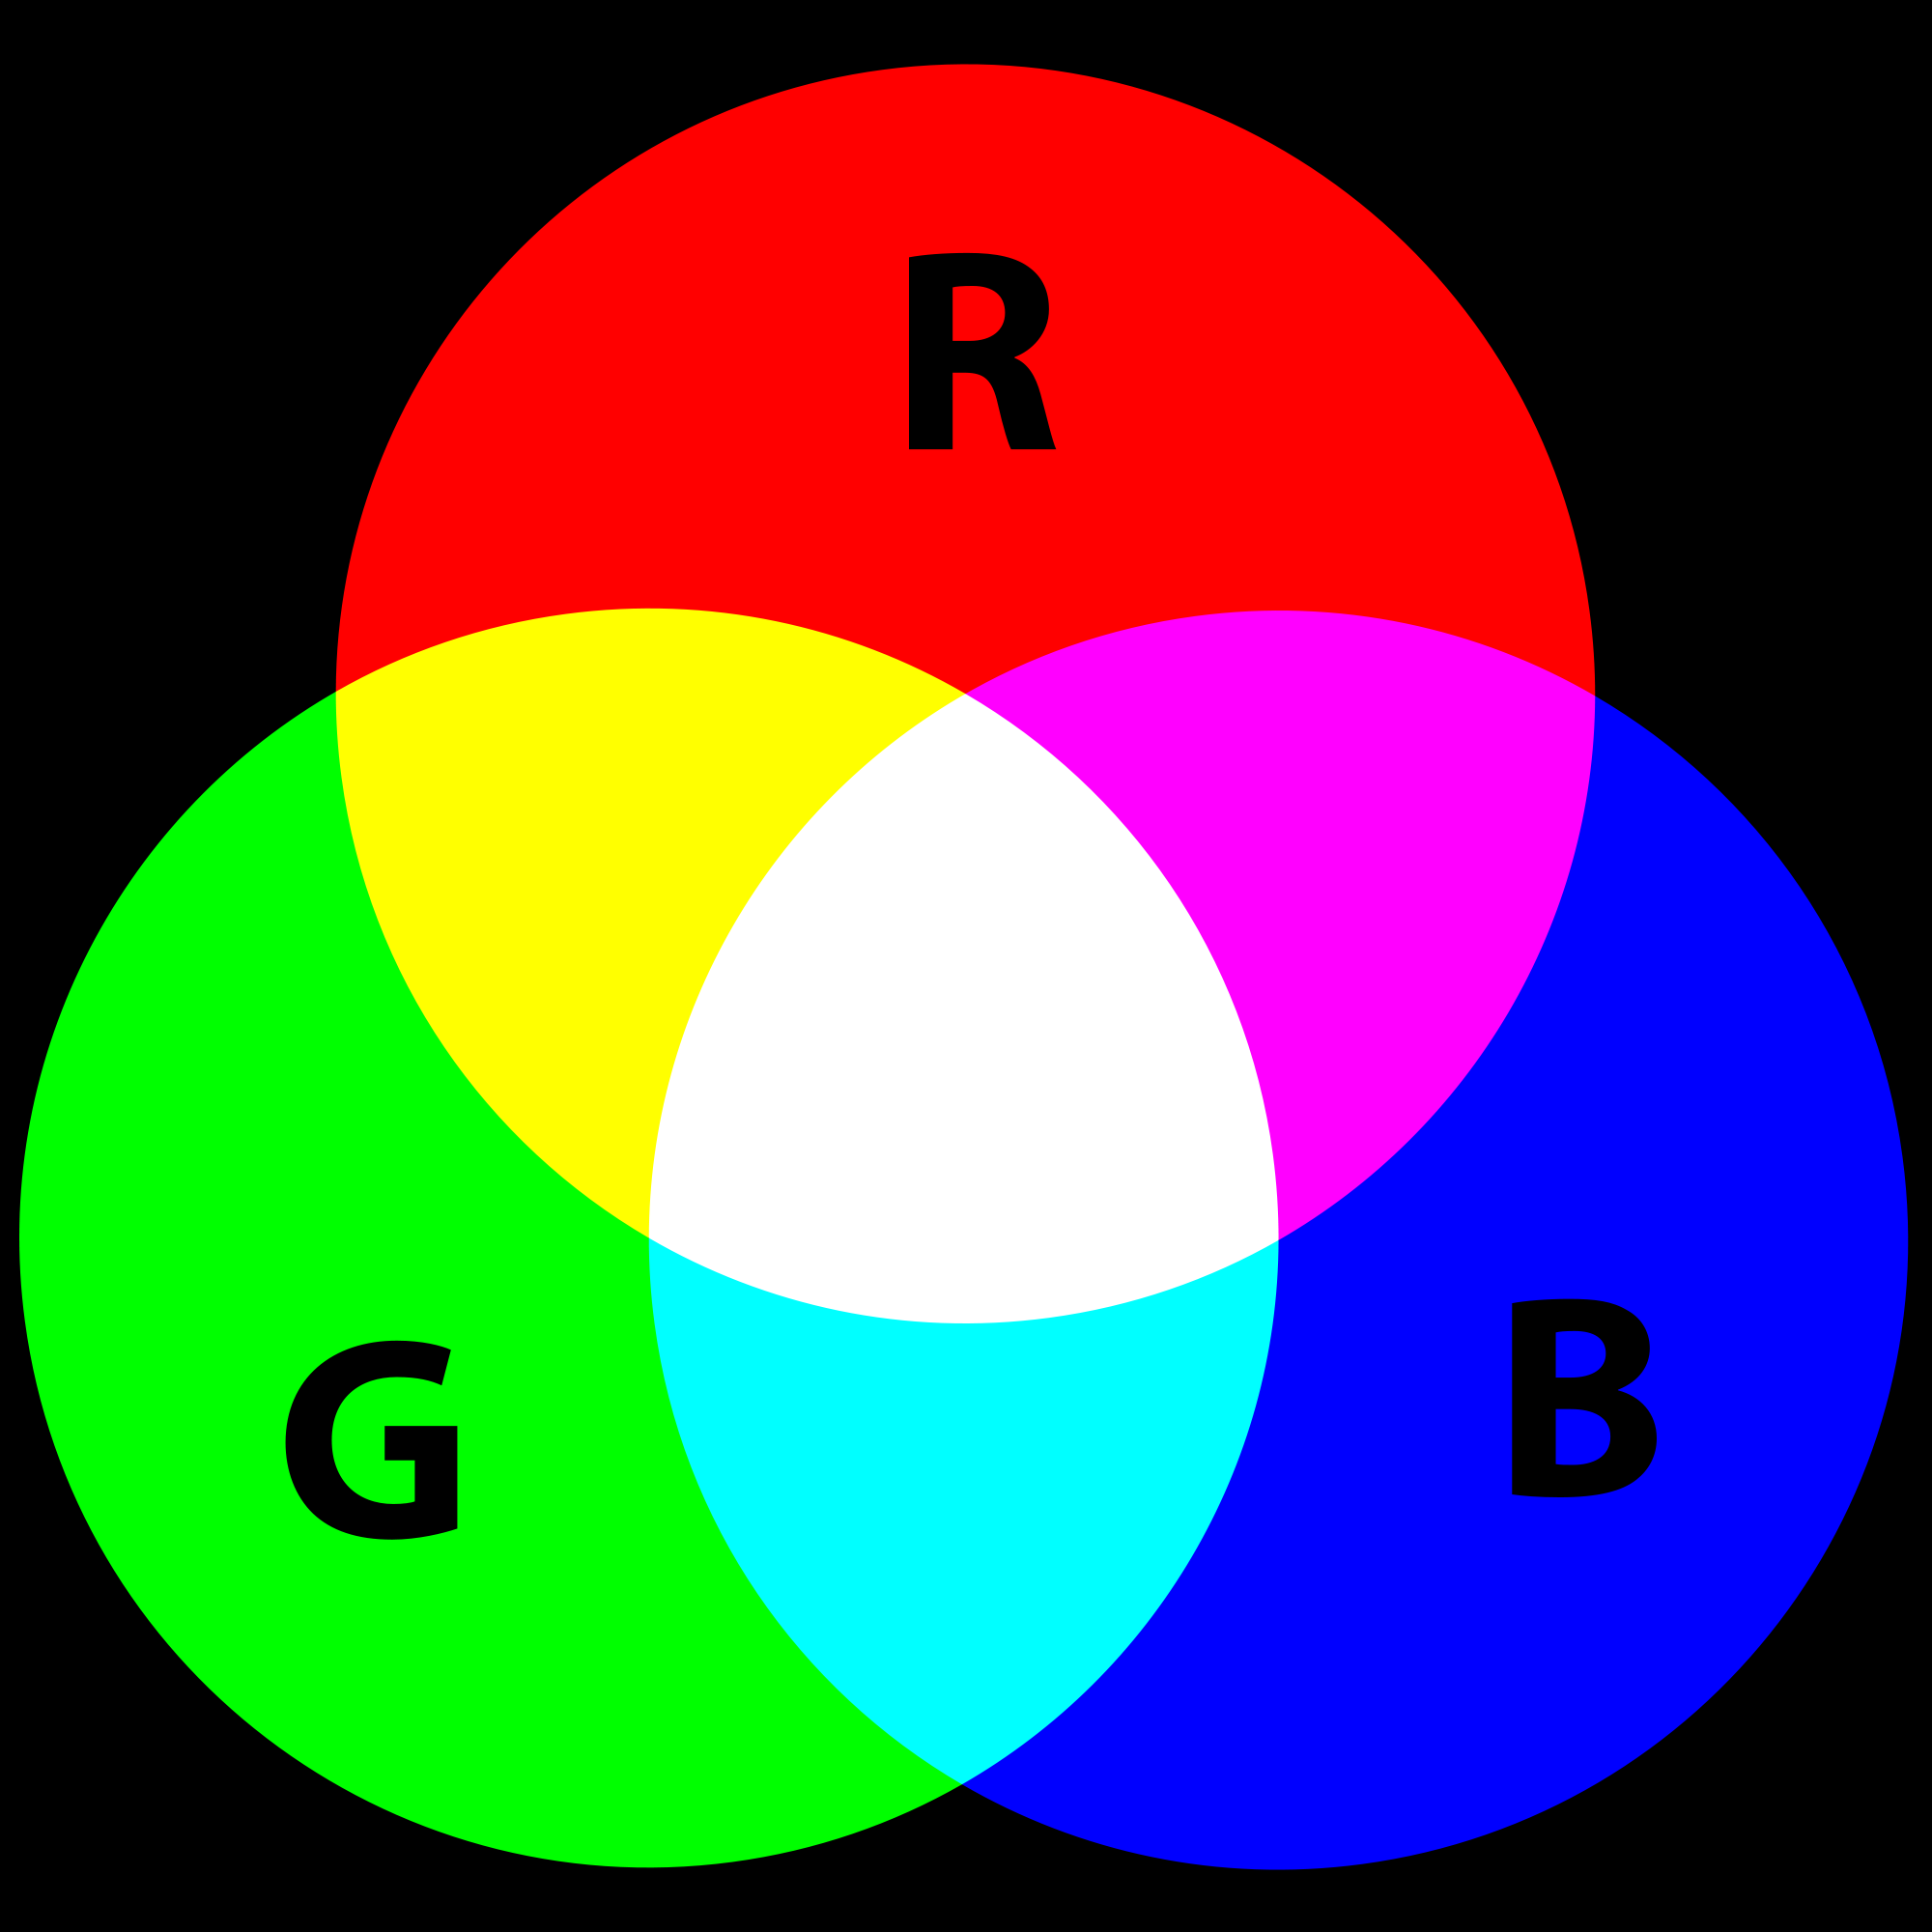
\includegraphics[width = 5cm]{rgb.png}
\caption{Colores Primarios}
\end{figure}

\subsection{Android.}
Es un sistema operativo inicialmente diseñado para teléfonos móviles. Fue creado por Android Inc. en el 2005 y posteriormente fue vendido a Google en 2007. Hoy en día este sistema operativo se encuentra en tablests, smartphones, televisiones e incluso en Hornos de Microondas y lavadoras. Está basado en Linux, que es un núcleo de sistema optativo libre gratuito y multiplataforma. \cite{Arias}
\newline
\begin{figure}[hbtp]
\centering

\includegraphics[width = 5cm]{android.png}
\caption{Mascota oficial de android}
\end{figure}

\subsection{Virus Informático}
Un virus informático en simplemente un programa informático, creado normalmente, con la finalidad de causar daño en el software del equipo destruyendo algunos o todos los archivos contenidos en un disco.\cite{Pardo}
\newline
\begin{figure}[hbtp]
\centering
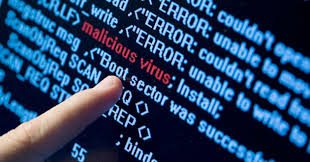
\includegraphics[width = 5cm]{virus.jpeg}
\caption{Codigo ejecutable de un programa virus}
\end{figure}

\subsection{Estado del Arte}
Una de las formas conocidas para esconder información es hacer uso del llamado Marca de agua. Este concepto es una técnica utilizada en la esteganografía. Con esta marca de agua se brinda seguridad para archivos tales como imágenes, software, video o audio. Esta técnica es utilizada por Patricia Jaimes y colaboradores en su trabajo titulado: “Una marca de agua inteligente aplicada al dinero electrónico”, para hacer que el dinero electrónico se vuelva invalido ante cualquier modificación. Este archivo de “dinero electrónico” no es amas que una imagen, pero no contiene un simple mensaje de validación, en lugar de eso se inserta código ejecutable que mantiene la integridad y autenticidad de la imagen.

Una de la desventaja que se puede presentar es la no aceptación por parte de los usuarios ya que estas marcas de agua como código ejecutable tienen las mismas características de los virus Informaticos llamados Perrun y Trojan. Los cuales fueron creados para demostrar que una imagen puede portar un virus y no ser detectado por un antivirus.
La técnica  de la marca de agua funciona de la siguiente manera: Un proveedor D utiliza una función de inserción E() la cual introduce un código C dentro de la imagen original I y como resultado se obtiene una imagen de código ejecutable, es decir: I = E(C).\cite{Jaimes}

Por otro lado, Yasuk Lim y colaboradores usaron un Sistema de Autentificación de Imágenes basado en Web usando una marca de agua frágil  con sistema embebido, es decir: un modelo cliente servidor. El sistema  de autenticación basado en web consiste en dos partes: uno es un sistema embebido de marca de agua y el otro es un sistema de autenticación. Quien tenga acceso al servidor puede generar imágenes de marca de agua y el envido o distribución de estas puede ser a través de protocolos de trasmisión de red tales como: FTP,  correo electrónico, etc.

El proceso comienza con una llave secreta que es usada para generar una función de valor vinario que depende de la clave. Esta función está basada en la técnica esteganográfica llamada: Ultimo byte significativo, es decir: LSB(Key, image).

El proceso de detección en una función inversa de LSB(key, image) para checar cada pixel, si hay una diferencia en cualquier pixel el servidor generara un mensaje de advertencia diciendo que la imagen puedo haber sido modificada o dañada. Toda esta información será generada en formato html. \cite{Yusuk}


%Fin del Capitulo 2
\section{Capítullo III: Metodología.}
Para este trabajo de investigación se ha usado la herramienta de desarrollo de aplicaciones para dispositivos móviles llamada eclipse, este es un IDE e cual es una buena herramienta para trabajar con dispositivos android. A sus vez, para el desarrollo de esta aplicación se ha hecho uso del lenguaje de programación java puesto que las aplicaciones android son escritas en java.

También una herramienta importante en este trabajo para simplificar muchas tareas y reducir tiempo es una librería escrita en java llamada JTransform la cual posee algoritmos para el cálculo de, tanto la  transformada discreta del coseno como la  trasformada rápida de Fourier, entre otras.

Las muestras empleadas en estas pruebas fueron recogidas a base de un dispositivo móvil (Smartphone)  el cual tiene la tarea de que con ayuda de quien lo maneja genere imágenes, o dicho de otra manera tomar fotografías, esta imagen va a ser la imagen portadora de información. Sin embargo la información que podrá portar es tan solo un mensaje pequeño el cual servirá de referencia para no perder la autenticidad de la imagen.
\newline
\begin{figure}[hbtp]
\centering
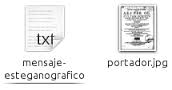
\includegraphics[width = 5cm]{portador.jpeg}
\caption{Imagen Portadora}
\end{figure}
\newline
Para alcanzar este objetivo los pasos que se tienen que llevar a cabo son:
\newline
Obtener la imagen portadora la cual estará compuesta por una matriz de NxM pixeles. Posteriormente convertir la matriz bidimensional en in  vector lineal de pixeles de longitud NxM. Con esta procedimiento se pretende un cálculo más rápido, ya que la transformada rápida de Fourier, o bien la transformada de Fourier discreta trabajan tanto en 3, 2 o solo una dimensión.
\newline
\begin{figure}[hbtp]
\centering
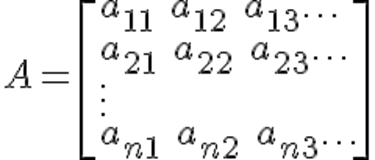
\includegraphics[width = 5cm]{matriz.png}
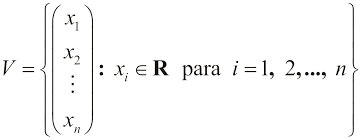
\includegraphics[width = 5cm]{vector.png}
\caption{Conversión de matriz a vector}
\end{figure}
\newline
Dado este vector x, se transforma con la trasformada rápida de Fourier obteniendo:
$X = DoubleFFT_1D(M*N).realForward(x)$, que es una clase de la librería JTransform. Teniendo un nuevo vector en el dominio de la frecuencia $X = (X_0, X_1, X_{MN})$.
\newline
Lo siguiente que se hace es que cada una de las letras ($c_i$) del mensaje culto, según su número de identificador en el código de ASCCI, convertirlas en Binario de tal manera que se tenga un conjunto de  caracteres: $c_i = (b_0, b_1,…,b_7)$ donde cada $b_i$ es un numero en binario de esa letra. y lo mismo sucede con cada uno de los pixeles $X_k$. Así, por ejemplo, para el primer $X_0$ el conjunto de números binarios seria: $(b_0, b_1,…,b_{31})$.
\newline
A continuación, se emplea la técnica del bit menos significativo (LSB), de tal manera que se intercambie el primer bit del primer carácter con el bit menos significativo del primer pixel $X_0$, el segundo bit del primer carácter con el bit menos significativo del segundo pixel $X_1$ y si para todos y cada uno de los bit que pertenecen a cada carácter.
\newline
\begin{figure}[hbtp]
\centering
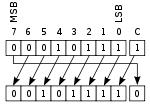
\includegraphics[width = 5cm]{lsb.png}
\caption{bit menos significativo}
\end{figure}
\newline
Finalmente se somete el nuevo vector $X_t$ a una transformada inversa obteniendo:
$x_t = DoubleFFT_1D(M*N).realInverse(X_t)$, donde $x$ no es igual $x_t$. De esa manera la calidad de la imagen transformada se percibe idéntica a la imagen original.
\newline
Para obtener el mensaje oculto se debe realizar nuevamente la transformaad rapida de Fourier y esta vez comparar los bits menos significativos como se especifico anterirmente. En caso de que uno y solo un bit difiera del resto del mensaje entonces eso quiere decir que la imagen pasó por una modificación hecha por un tercero. El mensaje se tiene que mantener intacto puesto que la FFT y la IFFT son procesos uno a uno, es decir procesos inversos ya que $x = IFFT(FFT(x))$.
\newline
Resumiendo estos procesos se puede observar los siguientes diagramas en donde se encuentran cada uno de los pasos descritos, tanto de la insercion del mensaje como la extraccion del mensaje.
\newline
\begin{figure}[hbtp]
\centering
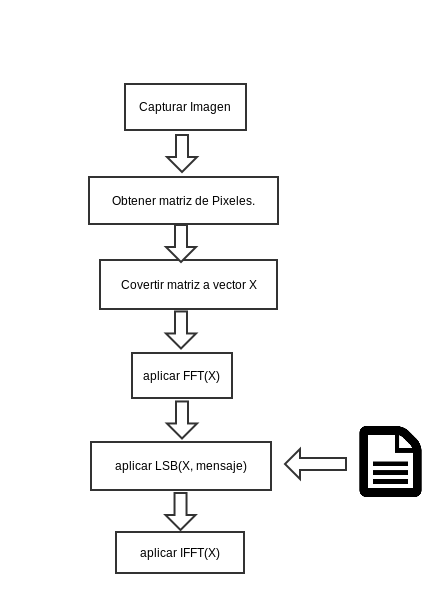
\includegraphics[width = 6cm]{algoritmoInsercion.png}
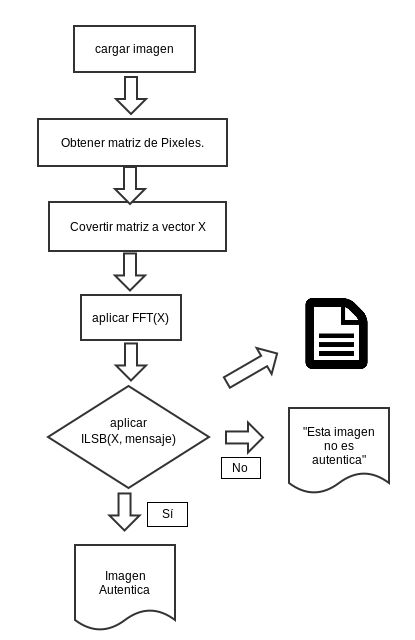
\includegraphics[width = 6cm]{algoritmoExtraccion.png}
\caption{Algoritmos de Inserción y de extracción}
\end{figure}
\newline
\section{Capitullo IV: Observaciones y experimentos.}
Dadas las estrategias expuestas anteriormente se tienen las siguientes imágenes obtenidas en cada uno de los pasos descritos, dados estos resultados  se pretende que el lector se convenza de que el método utilizado es lo suficiente eficaz para autenticar información y de la misma manera éste confíe en que no podría ser alterado por un tercero para fines maliciosos.
En primer lugar se tiene un ejemplo de una imagen recién producida por un  dispositivo con sistema operativo android (versión 2.3):
\newline
\begin{figure}[hbtp]
\centering
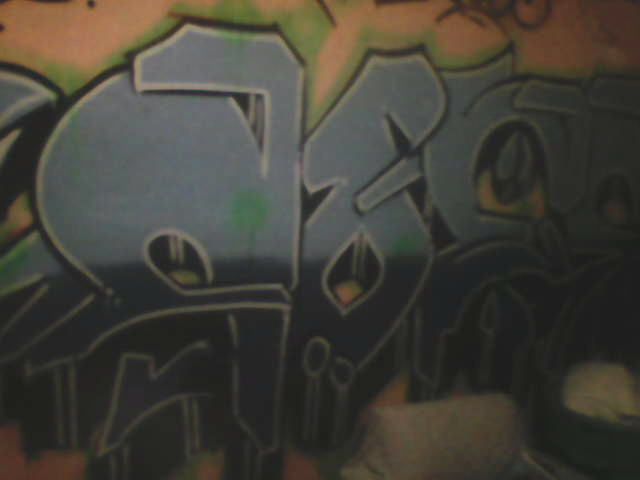
\includegraphics[width = 5cm]{chois0.png}
\caption{Imagen Original}
\end{figure}
\newline
Después de haber pasado por el proceso de transformación con la transformada rápida de Fourier se obtiene una imagen como esta:
\newline
\begin{figure}[hbtp]
\centering

\includegraphics[width = 5cm]{chois1.png}
\caption{Imagen transformada}
\end{figure}
\newline
En esta parte hay que hacer énfasis en que la imagen sufrió un cambio bastante radical puesto que no se percibe nada de la imagen original. Ahora bien, cuando se inserta el mensaje o se monta en este mapa de bits se podría decir que tampoco se incerto ningún mensaje, pero analizando los primeros 16 bits  de cada imagen se puede observar un cambio significativo , perro muy relevante:
\newline
\begin{figure}[hbtp]
\centering

\includegraphics[width = 5cm]{chois2.png}
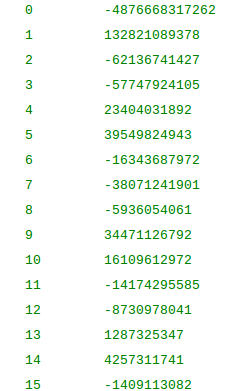
\includegraphics[width = 4cm]{selection1.png}
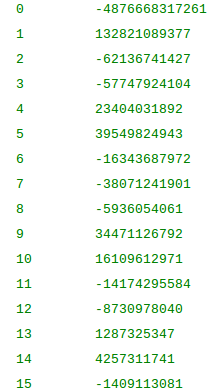
\includegraphics[width = 3.6cm]{selection2.png}
\caption{Imagen transformada con mensaje oculto}
\end{figure}
\newline
¿Por qué tanta insistencia en ocultar un mensaje usando FFT?. Si el mensaje se inserta bit a bit con el el metodo del bit menos significativo se obtiene el mismo resultado. La respuesta es sencilla: Una individuo con los suficientes conocimientos podría encontrar fácilmente el mensaje oculto, además la técnica del bit menos significativo no soporta compresiones y lo que se pretende es que el mensaje y la imagen comparta la misma persistencia durante toda su vida. Finalmente se muestra la imagen destransforma y con el mensaje insertado. 
\newline
\begin{figure}[hbtp]
\centering
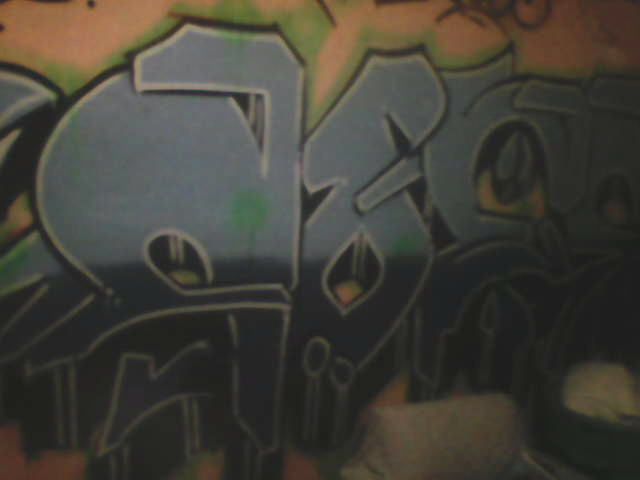
\includegraphics[width = 5cm]{chois3.png}
\caption{Imagen transformada y destransformada con mensaje oculto}
\end{figure}
\newline

Ahora se muestran algunas pruebas hechas durante el resarrollo de la aplicación:
\newline
\begin{figure}[hbtp]
\centering
\begin{tabular}{|p{3cm}|c|c|}
\hline
Descripcion & Imagen Original & Imagen Transformada\\
\hline
Cuando se inserta caracteres sin LSB (imagen 640x480) & 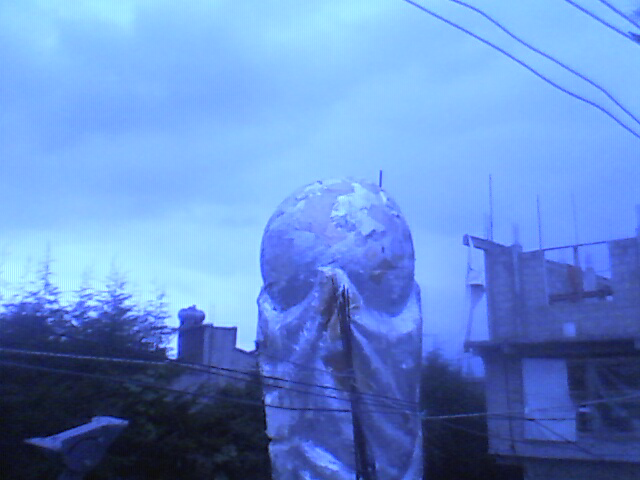
\includegraphics[width = 5cm]{hip0.png} & 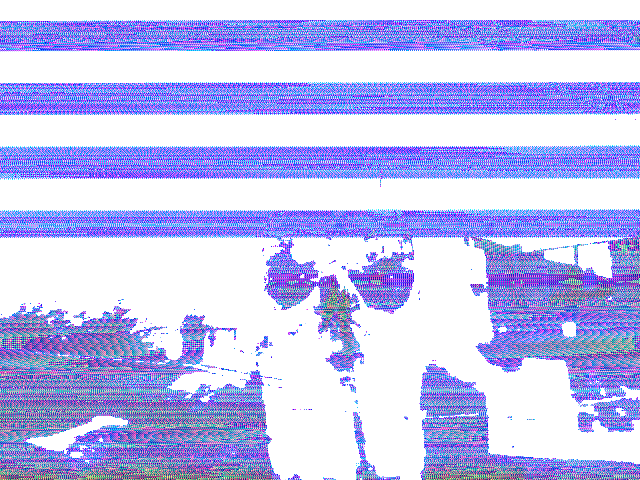
\includegraphics[width = 5cm]{hip1.png} \\
\hline
Cuando se insertan caracteres en matrices de 128x128 & 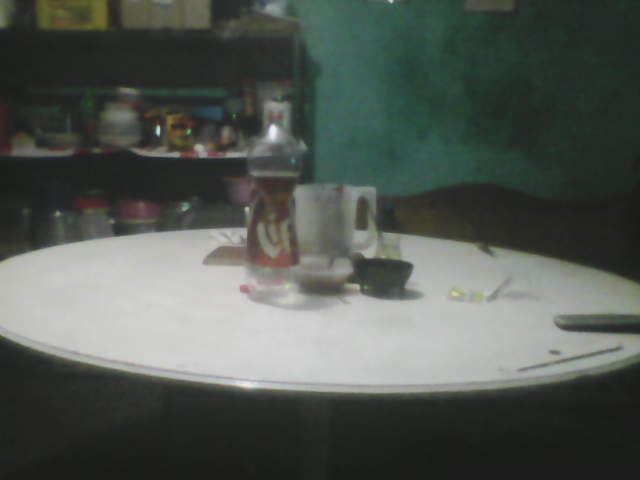
\includegraphics[width = 5cm]{flaw0.png} & 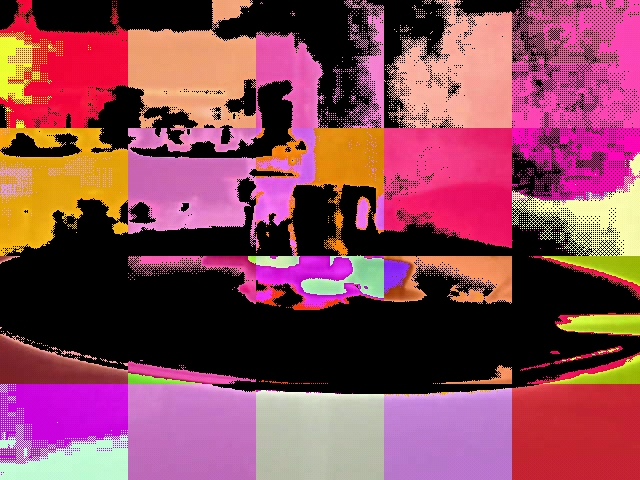
\includegraphics[width = 5cm]{flaw1.png} \\
\hline
Cuando se insertan caracteres usando FFT y LSB (imagen 640x480) & 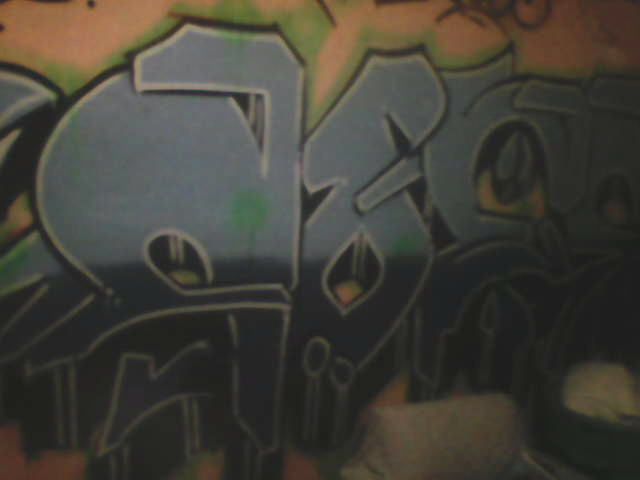
\includegraphics[width = 5cm]{chois0.png} & 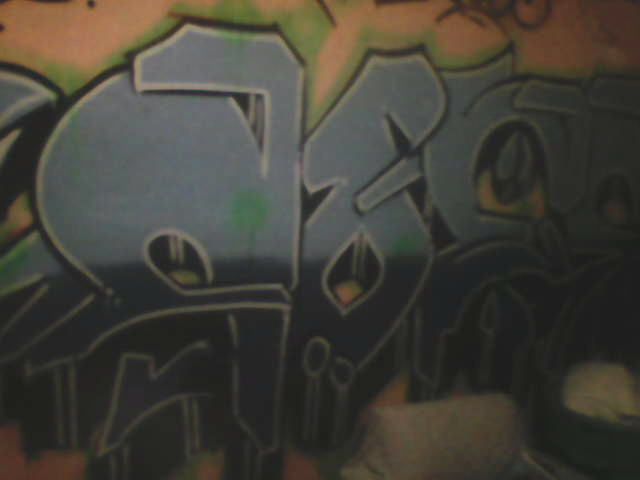
\includegraphics[width = 5cm]{chois3.png} \\
\hline
Cuando se insertan caracteres usando FFT y LSB (imagen 640x480) & 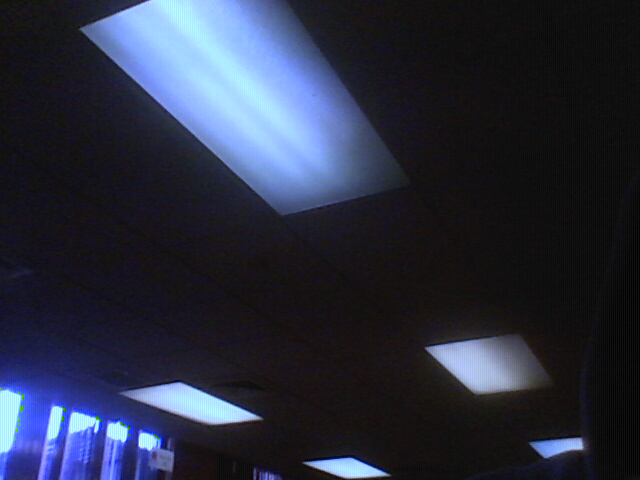
\includegraphics[width = 5cm]{psps0.png} & 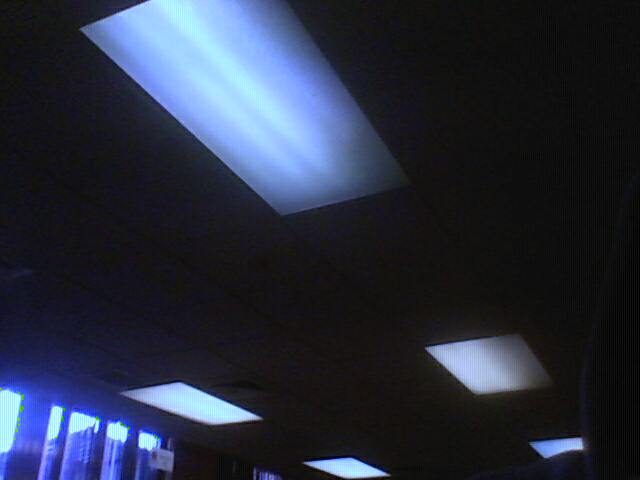
\includegraphics[width = 5cm]{psps1.png} \\
\hline
\end{tabular}
\caption{Resultados obtenidos}
\end{figure}
\newpage
\section{Capitullo V: Conclusiones y trabajos futuros.}
En este trabajo se implementó el algoritmo de la transformada de Fourier para ocultar un mensaje de texto en una imagen, el cual se implementó en un sistema operativo android.
Para probar la eficiencia del algoritmo de la transformada de Fourier se utilizaron diferentes imágenes con diferente resolución (128x128 y 640x480). Los resultados que se obtuvieron fueron con las imágenes de 640x480, como se pude ver en la figura 13.

Es importante mencionar que se continuará trabajando en el algoritmo de extraccion del mensaje .
\newpage
\bibliography{apa}{}
\bibliographystyle{apalike}

\end{document}